\section{SVM on Tree}
\label{sec:svm_on_tree}
\label{sec:svm_tree}

% [LE: Added comprehensive roadmap with cross-references]
In this section, we present a novel approach to binary classification using SVM on tree structures. Our method offers computational advantages in training classification model.

The section is organized as follows. We begin in \Cref{sec:tree-based-approximation} by constructing an augmented labeled tree from the training data that preserves essential geometric relationships. In \Cref{subsec:svm-model}, we formulate a SVM model on this tree structure, introducing concepts of noise functions and support pairs. \Cref{subsec:arbitrary-param} provides a general complexity analysis for arbitrary parameters, while \Cref{subsec:unit-param} establishes the crucial adjacency property for the unit parameter. \remLE{We should add complexity to the section of arbitrary lambda and unit lambda} %Finally, \Cref{subsec:algorithm} leverages these theoretical properties to propose efficient combinatorial algorithms with provable complexity bounds. 

\subsection{Tree-based approximation for data points}
\label{sec:tree-based-approximation}
Consider the classification problem with points $x_i\in \mathbb{R}^d$ and labels $y_i \in \{-1,+1\}$ for $i=1,\ldots, n$. 
We describe a procedure for constructing a tree that approximates the data points.

The idea is simple, we choose an arbitrary line, here we may consider the line joining the means of two groups, then for each data point $x_i$, we find its projection on line say $x'_i$. We then consider the tree including the path connecting the projection points and the edges connecting $(x_i, x'_i)$. We refer to this structure as the augmented tree approximating the data points. By augmented tree, we mean the tree obtained by augmenting the projection line with the edges connecting each data point to its projection.


We now detail how to construct the tree.
Let $\Delta$ be a line in $\mathbb{R}^d$. In this work, we focus on the line $\Delta$ connecting the two class means. For each $i=1,\ldots,n$, let $x'_i$ denote the orthogonal projection of $x_i$ onto $\Delta$. The tree is then built with vertices consisting of both the original points $x_i$ and their projections $x'_i$. Its edge set includes (i) spine edges, which are the line segments connecting consecutive projection points along $\Delta$, and (ii) spoke edges, which are the line segments connecting each original point $x_i$ to its projection $x'_i$. The details of this construction are described below.


Let $I_- = \{i\in \{1,..., n\} : y_i = -1\}$ and $I_+ = \{i \in \{1,..., n\} : y_i = +1\}$.
The class means is:
\begin{align*}
\mu_- &= \frac{1}{|I_-|}\sum_{i \in I_-} x_i, \\
\mu_+ &= \frac{1}{|I_+|}\sum_{i \in I_+} x_i.
\end{align*}

The unit vector pointing the direction of the line $\Delta$ conencting the two means is
\begin{equation*}
    w = \frac{\mu_+ - \mu_-}{\|\mu_+ - \mu_-\|_2}.
\end{equation*}

For each data point $x_i$, we compute its projection onto $\Delta$ passing through $\mu_-$ in direction $w$
\begin{equation}
x_i' = \mu_- + t_i w \text{ where } t_i = \langle x_i-\mu_-,\, w\rangle.
\end{equation}

The projected points $x_i'$ are then sorted by their projection coordinates $t_i$. Without loss of generality, we may assume that 
\begin{equation*}
    t_1 \leq \cdots \leq t_n. % [LE: Fixed ellipsis with \cdots for mathematical sequence]
\end{equation*}


We construct an augmented tree $T$ with vertex set
\begin{equation*}
V = \{x_1, \ldots, x_n\} \cup \{x'_1,\ldots, x'_n\}, % [LE: Fixed ellipsis in vertex set definition]
\end{equation*}
and edge set
\begin{equation*}
E = \{(x'_i, x'_{i+1}): i=1,\ldots, n-1\} \cup \{(x_i, x'_i): i=1,\ldots, n\}. % [LE: Fixed ellipsis in edge set definition]
\end{equation*}
% Since each $x_i$ has an associated label $y_i$, we also assign label $y_i$ for $x'_i$ for all $i=1,..., n$. In general, for $v\in V$, we write $L(v)$ for its label.
The tree $T$ is endowed with vertex labels and edge lengths as follows. Each $x_i$ and $x'_i$ inherits the original label $y_i$ for all $i=1,\ldots, n$. Each edge is assigned a length equal to the Euclidean distance between its endpoints. % [LE: Fixed ellipsis and typo in Euclidean] For any vertices $u,v \in V$, let $d(u,v)$ denote the distance between $u$ and $v$, defined as the total length of edges along the (unique) path connecting them.

We therefore referred to $T$ as labeled augmented tree. 
An illustration of this structure is shown in \Cref{fig:augmented-tree}. 
\remLE{The figure should be improved. 1) $x_i$ should be located in two sides of spine and 2) we should have positive vertices (black nodes), and negative vertices (white nodes).}


% The augmented tree $T$ is a connected graph structure that embeds both the original data points and their projections onto the separating direction. It consists of $2n$ vertices and $2n-1$ edges, forming a tree topology that preserves the geometric relationships between data points while enabling efficient tree-based computations.
% \textcolor{blue}{[LE: Added reference to the figure]} % [LE: Added reference to the figure]

We refer to edges connecting two adjacent projection points as \emph{spine edges}, and to edges connecting each original point with its projection as \emph{spoke edges}. The path formed by the sequence of all spine edges is called the \emph{spine} of the tree. \remLE{Check, if the concept of spine has not been used, we should remove it.}

\begin{figure}[htbp]
    \centering
    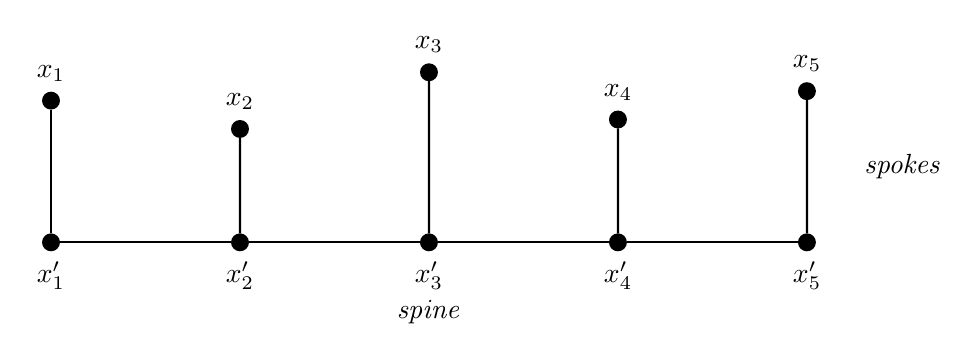
\begin{tikzpicture}[scale=1.2, thick]
        % Spine nodes (projections) - simple black circles
        \node[draw, circle, fill=black, inner sep=2pt, label=below:$x'_1$] (X1) at (0,0) {};
        \node[draw, circle, fill=black, inner sep=2pt, label=below:$x'_2$] (X2) at (2,0) {};
        \node[draw, circle, fill=black, inner sep=2pt, label=below:$x'_3$] (X3) at (4,0) {};
        \node[draw, circle, fill=black, inner sep=2pt, label=below:$x'_4$] (X4) at (6,0) {};
        \node[draw, circle, fill=black, inner sep=2pt, label=below:$x'_5$] (X5) at (8,0) {};
        
        % Original data points (perpendicular to spine)
        \node[draw, circle, fill=black, inner sep=2pt, label=above:$x_1$] (D1) at (0,1.5) {};
        \node[draw, circle, fill=black, inner sep=2pt, label=above:$x_2$] (D2) at (2,1.2) {};
        \node[draw, circle, fill=black, inner sep=2pt, label=above:$x_3$] (D3) at (4,1.8) {};
        \node[draw, circle, fill=black, inner sep=2pt, label=above:$x_4$] (D4) at (6,1.3) {};
        \node[draw, circle, fill=black, inner sep=2pt, label=above:$x_5$] (D5) at (8,1.6) {};
        
        % Spine edges
        \draw (X1) -- (X2) -- (X3) -- (X4) -- (X5);
        
        % Spoke edges (vertical connections)
        \draw (D1) -- (X1);
        \draw (D2) -- (X2);
        \draw (D3) -- (X3);
        \draw (D4) -- (X4);
        \draw (D5) -- (X5);
        
        % Labels for edge types
        \node[below] at (4,-0.5) {\emph{spine}};
        \node[right] at (8.5,0.8) {\emph{spokes}};
    \end{tikzpicture}
    \caption{Augmented tree structure showing original data points $x_i$ and their projections $x'_i$ onto the spine. The spine connects consecutive projections, while spoke edges connect each original point to its projection.}
    \label{fig:augmented-tree}
\end{figure}



Having constructed the augmented tree that embeds our data points while preserving their geometric relationships, we now formulate a SVM model that operates directly on this tree structure. This model will leverage the tree's connectivity to define support vectors and decision boundaries in a computationally efficient manner. % [LE: Added transition to SVM model section]

\subsection{SVM model on tree}
\label{subsec:svm-model}
\remLE{missing definition of $V_-, V_+, V_+(u, v)$ and $V_-(u, v)$.}

From classical SVM theory, we know that the formulation of the SVM model strongly relies on the support vectors, which are points with different labels. % [LE: Fixed XXX reference to classical SVM theory]
Let $T$ be the tree constructed in \Cref{sec:tree-based-approximation}.
We focus on a pair of vertices with different labels, say 
\begin{equation*}
    u \in V_+ \text{ and } v \in V_-,
\end{equation*}
which is the analog of support vectors in the tree context.
We seek such pairs of nodes satisfying two criteria. \remLE{First is to maximize the margin, second is to to minimize the loss. In the following, we will model these two quantities.}

First, the margin in the classical SVM is modeled as the distance between two support nodes, say $d(u,v)$.

Second, we introduce the notion of noisy nodes in the tree.
Given a support pair $(u,v)$ with $u \in V_+$ and $v \in V_-$, noisy nodes are vertices that lie on the path between $u$ and $v$ \remLE{not correct} but have the same label as one of the endpoints. These nodes contribute to classification errors and must be penalized in our objective function. \textcolor{blue}{[LE: Added formal definition of noisy nodes concept]} % [LE: Added formal definition of noisy nodes concept]

Consider a positive support node $u$, and among the subtrees rooted at $u$, take the branch containing the negative node $v$.
We regard the positive nodes on the same branch as $v$ as positive noisy nodes.
This motivates the definition of the set of positive noisy nodes, denoted by $V_+(u,v)$, as the set of positively labeled vertices in the subtree on the branch rooted at $u$ toward $v$.
Similarly, we define $V_-(v,u)$ as the set of negatively labeled vertices on the branch rooted at $v$ toward $u$, referred to as negative noisy nodes.
\remLE{Merge above two paragraphs.}

We define the positive and negative noise function of $u$ and $v$ as follows:
\begin{align}
f_+(u,v) &= \sum_{z\in V_+(u,v)} d(z,u), \\
f_-(v,u) &= \sum_{z\in V_-(v,u)} d(z,v).
\end{align}
It is important to note that the order of variable is important here, with $u\in V_+$ in the first location in $f_+$, while $v \in V_-$ in the first location in $f_-$.
The total noise is
\begin{equation*}
    f(u,v) = f_+(u,v) + f_-(v,u)
\end{equation*}
% Note that the order of $(u, v)$ is important in the noise function $f(u,v)$, while not important in the distance function $d(u,v)$. % [LE: Replaced XXX with specific function references]

% We define the margin as the distance between two support vectors
% \begin{equation*}
%     d(u,v).
% \end{equation*}
Since we aim to minimize the noise while maximizing the margin, we define the total loss function 1as
\begin{equation*}
    L_\lambda(u,v) = f(u,v) - \lambda \cdot d(u,v).
\end{equation*}
where $\lambda \geq 0$ is a parameter which controls the balance between the noise and the margin.

We define a support pair $(u, u)$, analogous to the support vectors in standard SVMs, as the pair of oppositely labeled nodes minimizing $L_\lambda(u,v)$. The \emph{decision boundary} corresponding to a support pair $(u, v)$ is the perpendicular bisector hyperplane of the segment between $u$ and $v$ in $\mathbb{R}^d$. 

\begin{figure}[htbp]
    \centering
    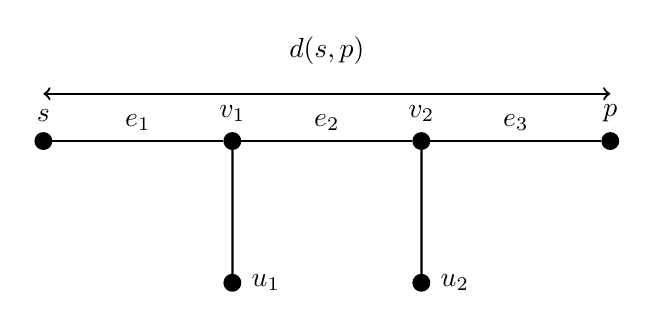
\begin{tikzpicture}[scale=1.2, thick]
        % Support nodes and path nodes
        \node[draw, circle, fill=black, inner sep=2pt, label=above:$s$] (S) at (0,0) {};
        \node[draw, circle, fill=black, inner sep=2pt, label=above:$v_1$] (V1) at (2,0) {};
        \node[draw, circle, fill=black, inner sep=2pt, label=above:$v_2$] (V2) at (4,0) {};
        \node[draw, circle, fill=black, inner sep=2pt, label=above:$p$] (P) at (6,0) {};
        
        % Additional nodes in subtrees
        \node[draw, circle, fill=black, inner sep=2pt, label=right:$u_1$] (U1) at (2,-1.5) {};
        \node[draw, circle, fill=black, inner sep=2pt, label=right:$u_2$] (U2) at (4,-1.5) {};
        
        % Tree edges
        \draw (S) -- (V1) -- (V2) -- (P);
        \draw (V1) -- (U1);
        \draw (V2) -- (U2);
        
        % Distance annotation
        \draw[<->, thick] (0,0.5) -- (6,0.5);
        \node[above] at (3,0.7) {$d(s,p)$};
        
        % Edge labels
        \node at (1,0.2) {$e_1$};
        \node at (3,0.2) {$e_2$};
        \node at (5,0.2) {$e_3$};
    \end{tikzpicture}
    \caption{Support pair illustration showing nodes $s$ and $p$ connected by a path with intermediate vertices and subtree nodes. \remLE{Fix the figure, $s$ and $p$ should not be the leaves.}}
    \label{fig:support-pair}
\end{figure}




Once a suport pair has been found, we can make prediction for new data point. Given a new data point $x_{new}$, we classify it by determining which side of the decision boundary it lies on. Specifically, if the hyperplane bisecting the segment between support vectors $s$ and $p$ has normal vector $\vec{n} = p - s$ and passes through the midpoint $\frac{s + p}{2}$, then we classify $x_{new}$ as positive if $\langle x_{new} - \frac{s + p}{2}, p - s \rangle > 0$ and negative otherwise. \remLE{Quite complex rule and not intuitive, Rewrite it like: If $x_{new}$ and $u$ are in the same side--> positive label. Use $u, v$ instead of $s, p$.}

With our SVM model on tree now formulated, we turn to the computational challenges of training such a model. The key question is how to efficiently find the optimal support pair that m1inimizes the loss function. We first analyze the general case for arbitrary parameter values, then focus on the special case $\lambda=1$ which admits significant theoretical and computational simplifications. 

\subsection{Training SVM model on tree with arbitrary parameter}
\label{subsec:arbitrary-param}

By definition of SVM model on tree, the naive training approach for  such a model needs the evaluation of objectives for all pairs of nodes. Since there are $O(n^2)$ support pairs and $O(n)$ time for computing the objective, the overall complexity for such naive approach is $O(n^3)$.

However, in this subsection, we can significantly reduce this complexity by dynamic programming. In the following, we first describe the preprocessing step. After that, we will show how to reduce the overall complexity to $O(n^2)$.

\remLE{Preprocessing step}
% \subsubsection{Preprocessing} 
% \label{sec:preprocessing} % [LE: Added section label for reference] 

Recall $x'_1, \ldots,x'_n$ are projections of $x_1,\ldots, x_n$ and we assume that $x'_1, \ldots,x'_n$ have been sorted in a certain order, \eg by their first coordinates. By the adjacency property (Theorem~\ref{thm:adjacency}), we know that support vectors form a pair $(x'_i, x'_{i+1})$ with opposite signs. % [LE: Fixed ellipsis and XXX reference] The margin is clearly $d(x'_i, x'_{i+1}) = \|x'_i - x'_{i+1}\|_2$.
To compute the total loss, we only need $f(x'_i, x'_{i+1})$ for $i=1,.., n-1$. In the following, we will clarify how to compute these values efficiently using dynamic programming.


For $i = 1, \ldots, n-1$, we define data at iteration $i$ as % [LE: Fixed ellipsis]
\begin{align*}
    N^{>i}_+  & = |\{v \in V_+(x'_i, x'_{i+1})\}| = 2 |\{j > i: y_j=+1\}|\\
    N^{>i}_-  & = |\{v \in V_-(x'_i, x'_{i+1})\}| = 2 |\{j > i: y_j=-1\}|\\
    N^{\leq i}_+  & = |\{v \in V_+(x'_{i+1}, x'_{i})\}| = 2 |\{j \leq  i: y_j=+1\}|\\
    N^{\leq i}_-  & = |\{v \in V_+(x'_{i+1}, x'_{i})\}| = 2 |\{j \leq  i: y_j=-1\}|
\end{align*}
and
\begin{align*}
    d^{>i}_+  & = \sum_{v \in V_+(x'_i, x'_{i+1})} d(x'_i, v)
    & = \sum_{j > i, y_j = +1 }[d(x'_i, x'_j) + d(x'_i, x_j)],\\
    d^{>i}_-  & = \sum_{v \in V_-(x'_i, x'_{i+1})} d(x'_i, v)
    & = \sum_{j > i, y_j = -1 }[d(x'_i, x'_j) + d(x'_i, x_j)],\\
    d^{\leq i}_+  & = \sum_{v \in V_+(x'_{i+1}, x'_{i})} d(v, x'_{i+1})
    & = \sum_{j \leq i, y_j = +1 }[d(x'_j, x'_{i+1}) + d(x_j, x'_{i+1})]\\
    d^{\leq i}_-  & = \sum_{v \in V_-(x'_{i+1}, x'_{i})} d(v, x'_{i+1})
    & = \sum_{j \leq i, y_j = -1 }[d(x'_j, x'_{i+1}) + d(x_j, x'_{i+1})].
\end{align*}

Consider $i = 1, \ldots, n-1$. If $y_i = -1$ and $y_{i+1}=+1$, we then have % [LE: Fixed ellipsis] 
\begin{equation*}
    f(x'_i, x'_{i+1}) = d^{>i}_- + d^{\leq i}_+.
\end{equation*}
Otherwise, $y_i = +1$ and $y_{i+1}=-1$, then 
\begin{equation*}
    f(x'_i, x'_{i+1}) = d^{>i}_+ + d^{\leq i}_-.
\end{equation*}

Therefore, to compute the total noise function, we should have an efficient method to compute $(d^{>i}_+, d^{>i}_-, d^{\leq i}_+, d^{\leq i}_-)$. This can be achived using the dynamic updates.

The following proposition claims that how the information of $N^{\leq i}_-$ and $d^{\leq i}_-$ can be used to derive  $N^{\leq i+1}_-$ and $d^{\leq i+1}_-$ efficiently. The proof of the proposition will show the procedure in details.

\begin{proposition}
    For $i=1,\ldots, n-1$, if we have $N^{\leq i}_-$ and $d^{\leq i}_-$, then we can update $N^{\leq i+1}_-$ and $d^{\leq i+1}_-$ in constant time. % [LE: Fixed ellipsis]
\end{proposition}
\begin{proof}
    By definition,
    \[
        d^{\leq i}_- = \sum_{\substack{j \le i \\ y_j=-1}} \big( d(x'_j, x'_{i+1}) + d(x_j, x'_{i+1}) \big),\qquad
        d^{\leq i+1}_- = \sum_{\substack{j \le i+1 \\ y_j=-1}} \big( d(x'_j, x'_{i+2}) + d(x_j, x'_{i+2}) \big).
    \]
    First consider the sum over indices $j \le i$ with $y_j=-1$. Due to the tree structure consisting of the spine (connecting the $x'_k$ in order) and spokes (connecting each $x_k$ to its projection $x'_k$), for all $j \le i$, the unique path from $x'_j$ (or $x_j$) to $x'_{i+2}$ passes through $x'_{i+1}$. Therefore,
    \[
        d(x'_j, x'_{i+2}) = d(x'_j, x'_{i+1}) + d(x'_{i+1}, x'_{i+2}),\qquad
        d(x_j,  x'_{i+2}) = d(x_j,  x'_{i+1}) + d(x'_{i+1}, x'_{i+2}).
    \]
    Summing over all $j \le i$ with $y_j=-1$, the increase due to shifting the anchor from $x'_{i+1}$ to $x'_{i+2}$ is
    \[
        N^{\le i}_- \cdot d(x'_{i+1}, x'_{i+2}),
    \]
    since $N^{\le i}_-$ counts exactly the number of negative vertices participating in the sum (each index $j$ contributes two vertices $x'_j$ and $x_j$).

    Additionally, if $y_{i+1}=-1$, two new vertices appear in the region $\le i+1$, namely $x'_{i+1}$ and $x_{i+1}$. Their contribution to $d^{\le i+1}_-$ is
    \[
        d(x'_{i+1}, x'_{i+2}) + d(x_{i+1}, x'_{i+2})
        = d(x'_{i+1}, x'_{i+2}) + \big( d(x_{i+1}, x'_{i+1}) + d(x'_{i+1}, x'_{i+2}) \big)
        = 2\,d(x'_{i+1}, x'_{i+2}) + d(x_{i+1}, x'_{i+1}).
    \]
    Combining both parts, we obtain the update formulas for the two cases based on the label $y_{i+1}$:
    \begin{align*}
        N^{\le i+1}_- &= \begin{cases}
            N^{\le i}_- + 2, & \text{if } y_{i+1}=-1,\\
            N^{\le i}_-, & \text{if } y_{i+1}=+1,
        \end{cases}\\[4pt]
        d^{\le i+1}_- &= \begin{cases}
            d^{\le i}_- + N^{\le i}_-\, d(x'_{i+1}, x'_{i+2}) + 2\,d(x'_{i+1}, x'_{i+2}) + d(x_{i+1}, x'_{i+1}), & \text{if } y_{i+1}=-1,\\
            d^{\le i}_- + N^{\le i}_-\, d(x'_{i+1}, x'_{i+2}), & \text{if } y_{i+1}=+1.
        \end{cases}
    \end{align*}
    Clearly, each update step only uses quantities known at step $i$ and distances between consecutive spine points, so it can be performed in constant time. Therefore, knowing $N^{\le i}_-$ and $d^{\le i}_-$ is sufficient to update $N^{\le i+1}_-$ and $d^{\le i+1}_-$.
\end{proof}

Extending above proposition, we obtain the following result.
\begin{proposition}
    We can compute the following quantities in $O(n)$.
    \begin{enumerate}
        \item $(N^{>i}_+, N^{>i}_-, N^{\leq i}_+, N^{\leq i}_-)$ for all $i=1,\ldots, n-1$ % [LE: Fixed ellipsis]
        \item $(d^{>i}_+, d^{>i}_-, d^{\leq i}_+, d^{\leq i}_-)$ for all $i=1,\ldots, n-1$ % [LE: Fixed ellipsis]
        \item $f(x'_i, x'_{i+1})$ for all $i=1,\ldots, n-1$. % [LE: Fixed ellipsis]
    \end{enumerate}
\end{proposition}
\begin{proof}
    We prove this by applying Proposition 5.1 systematically, using the dynamic programming technique on trees. % [LE: Fixed XXX reference to specific proposition about constant-time updates]

    \textit{Step 1: Computing all counting quantities in $O(n)$.}
    The counting quantities can be computed by simple linear scans:
    \begin{itemize}
        \item $N^{>i}_+, N^{>i}_-$: Scan from right to left, counting positive/negative labels.
        \item $N^{\leq i}_+, N^{\leq i}_-$: Scan from left to right, counting positive/negative labels.
    \end{itemize}
    Each quantity is updated in $O(1)$ per position, giving total $O(n)$ time.

    \textit{Step 2: Computing all distance quantities in $O(n)$.}
    This is where we apply the dynamic programming approach described above. The key insight is that our augmented tree has a spine structure, which allows efficient re-rooting operations. % [LE: Replaced XXX with specific reference to DP approach]

    Left-to-right pass for computing $d^{\leq i}_+, d^{\leq i}_-$: % [LE: Verified indices are correct for progressive accumulation]
    \begin{itemize}
        \item Initialize: $d^{\leq 1}_+ = 2d(x'_1, x'_2) + d(x_1, x'_2)$ if $y_1 = +1$, else $0$.
        \item For $i = 1, \ldots, n-2$: Apply Proposition 1 (and its symmetric version for positive labels) to update $d^{\leq i+1}_\pm$ from $d^{\leq i}_\pm$ in $O(1)$ time.
    \end{itemize}

    Right-to-left pass for computing $d^{>i}_+, d^{>i}_-$:
    \begin{itemize}
        \item Initialize: $d^{>n-1}_+ = 0, d^{>n-1}_- = 0$ (no points beyond position $n-1$).
        \item For $i = n-1, n-2, \ldots, 2$: Use the symmetric update formula to compute $d^{>(i-1)}_\pm$ from $d^{>i}_\pm$ in $O(1)$ time.
    \end{itemize}

    The symmetric update formula for the right-to-left pass is obtained by reversing the roles: when moving from anchor $x'_{i+1}$ to $x'_i$, all points $j > i$ have their distances increased by $d(x'_i, x'_{i+1})$, and if $y_i = -1$, we add the contribution of the new point $i$.

    \textit{Step 3: Computing $f(x'_i, x'_{i+1})$ in $O(n)$.}
    Once all counting and distance quantities are computed, we can evaluate $f(x'_i, x'_{i+1})$ for each $i = 1, \ldots, n-1$ using the formulas given in the preprocessing section. % [LE: Replaced XXX with specific section reference]
    % \begin{itemize}
    %     \item If $y_i = -1, y_{i+1} = +1$: $f(x'_i, x'_{i+1}) = d^{>i}_- + d^{\leq i}_+$.
    %     \item If $y_i = +1, y_{i+1} = -1$: $f(x'_i, x'_{i+1}) = d^{>i}_+ + d^{\leq i}_-$.
    % \end{itemize}
    Each evaluation takes $O(1)$ time, giving total $O(n)$ time.

    % \textbf{Conclusion:} By Proposition 5.3 (dynamic programming on trees), the re-rooting operations along the spine can be performed efficiently. Since each of the three steps requires $O(n)$ time, the total time complexity is $O(n)$.
\end{proof}



\remLE{Complexity analysis here}

\begin{theorem}
    For any $\lambda \geq 0$, we can find the support nodes in $O(n^2)$.
\end{theorem}

\textbf{Proof idea:} The key insight is that while the distance matrix on tree can be computed in $O(n^2)$ time, the noise function $f(u, v)$ can also be computed in $O(n^2)$ time for all pairs by leveraging dynamic programming on the tree structure. This eliminates the need for $O(n^3)$ pairwise evaluations.\remLE{I think we should clarify how to do dynamic programming here, based on the preprocessing steps.}

While the general case admits an $O(n^2)$ algorithm, we can achieve even more significant improvements by focusing on the special case $\lambda=1$. This parameter choice leads to a remarkable structural property that dramatically reduces the search space and enables linear-time preprocessing algorithms. 

\subsection{Training SVM model on tree with unit parameter}
\label{subsec:unit-param}

% \subsubsection{Adjacency property for unit parameter}



% \begin{figure}[htbp]
%   \centering
%   \begin{tikzpicture}[scale=1.5, thick]
%     % Vertices
%     \node[draw, circle, fill=black, inner sep=2pt, label=above:$p_4$] (P4) at (0,0) {};
%     \node[draw, circle, fill=black, inner sep=2pt, label=above:$s$] (S) at (2,0) {};
%     \node[draw, circle, fill=black, inner sep=2pt, label=above:$p_2$] (P2) at (4,0) {};
%     \node[draw, circle, fill=black, inner sep=2pt, label=above:$p_1$] (P1) at (6,0) {};
%     \node[draw, circle, fill=black, inner sep=2pt, label=below:$p_3$] (P3) at (4,-1.5) {};

%     % Edges with labels
%     \draw (P4) -- node[above] {$z$} (S);
%     \draw (S) -- node[above] {$x$} (P2);
%     \draw (P2) -- node[above] {$y$} (P1);
%     \draw (P2) -- (P3);
%   \end{tikzpicture}
%   \caption{Tree structure illustrating nodes $s$, $p_1$, $p_2$, $p_3$, and $p_4$ with edge weights $x$, $y$, and $z$.}
%   \label{fig:tree_nodes}
% \end{figure}


In this subsection, we establish a key theoretical properties of our SVM on tree formulation, focusing on the case $\lambda=1$. Specifically, we show that the two support nodes are adjacent and lies on the spine of the tree. 

\textbf{Definition (Spine):} The spine of the augmented tree $T$ is the path connecting all projected points $x'_1, x'_2, \ldots, x'_n$ in their sorted order along the direction $w$. This forms the main backbone of our tree structure, with each original data point $x_i$ connected to its projection $x'_i$ via a spoke edge. \remLE{Already define}

This fundamental property significantly reduces the search space for optimal support pairs. \remLE{remove this sentence?!}


Let $s \in V_+$ and $p_1, p_2\in V_-$ such that $p_2$ is in the path connecting $s$ and $p_1$, \ie
\begin{equation}
    d(s, p_1) = d(s, p_2) + d(p_2, p_1)
    \label{eq:distance-decomposition}
\end{equation}

Define the \emph{residual} of vertex set 
\begin{equation*}
    R = V_-(p_1, s) \setminus V_-(p_2, s).
\end{equation*}
The residual set $R$ represents the set of negatively labeled vertices that are in the noisy region for the pair $(s, p_1)$ but not for the pair $(s, p_2)$. Since $p_2$ lies on the path from $s$ to $p_1$, the set $R$ consists of vertices that become "newly included" in the noisy region when we extend the boundary from $p_2$ to $p_1$. This set is crucial for analyzing the difference in noise functions between different support pairs. %\textcolor{blue}{[LE: Added formal definition of residual set concept]} % [LE: Added formal definition of residual set concept]

Please refer to \Cref{fig:diff-set} for an illustration of the residual set $R$. % [LE: Removed the Vietnamese comment and added proper description] 

\begin{figure}[h!]
    \centering
    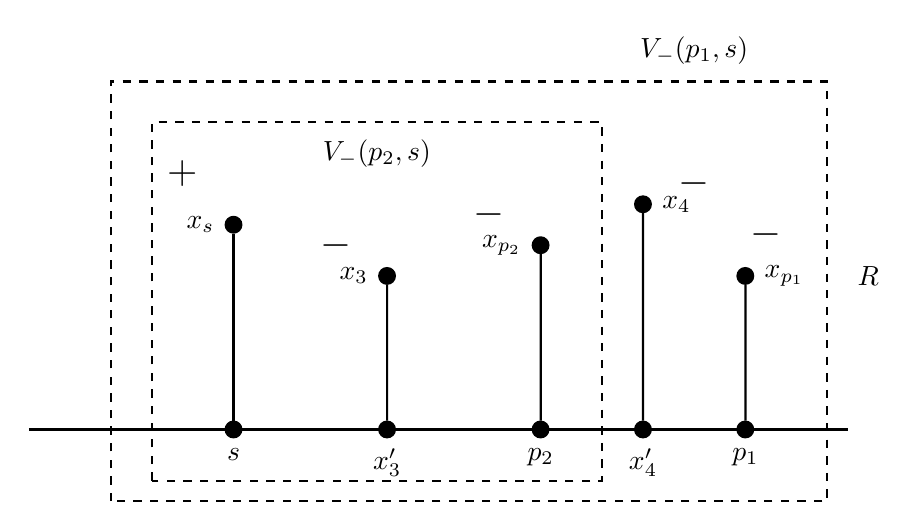
\begin{tikzpicture}[scale=1.3, thick]
        % Spine (horizontal line)
        \draw[thick] (0,0) -- (8,0);
        
        % Projections on spine
        \node[draw, circle, fill=black, inner sep=2pt, label=below:$s$] (S) at (2,0) {};
        \node[draw, circle, fill=black, inner sep=2pt, label=below:$p_2$] (P2) at (5,0) {};
        \node[draw, circle, fill=black, inner sep=2pt, label=below:$p_1$] (P1) at (7,0) {};
        
        % Original points (spokes)
        \node[draw, circle, fill=black, inner sep=2pt, label=left:$x_s$] (XS) at (2,2) {};
        \node[draw, circle, fill=black, inner sep=2pt, label=left:$x_{p_2}$] (XP2) at (5,1.8) {};
        \node[draw, circle, fill=black, inner sep=2pt, label=right:$x_{p_1}$] (XP1) at (7,1.5) {};
        
        % Some additional negative points
        \node[draw, circle, fill=black, inner sep=2pt, label=left:$x_3$] (X3) at (3.5,1.5) {};
        \node[draw, circle, fill=black, inner sep=2pt, label=right:$x_4$] (X4) at (6,2.2) {};
        
        % Projections of additional points
        \node[draw, circle, fill=black, inner sep=2pt, label=below:$x'_3$] (X3P) at (3.5,0) {};
        \node[draw, circle, fill=black, inner sep=2pt, label=below:$x'_4$] (X4P) at (6,0) {};
        
        % Spokes (connections)
        \draw (S) -- (XS);
        \draw (P2) -- (XP2);
        \draw (P1) -- (XP1);
        \draw (X3P) -- (X3);
        \draw (X4P) -- (X4);
        
        % Class labels - positioned in clear areas away from dashed lines
        \node[font=\Large] at (1.5,2.5) {$+$};
        \node[font=\Large] at (4.5,2.1) {$-$};
        \node[font=\Large] at (7.2,1.9) {$-$};
        \node[font=\Large] at (3.0,1.8) {$-$};
        \node[font=\Large] at (6.5,2.4) {$-$};
        
        % Region V-(p2, s) - expanded with more space
        \draw[dashed, thick] (1.2,-0.5) -- (1.2,3.0) -- (5.6,3.0) -- (5.6,-0.5) -- cycle;
        \node[font=\normalsize] at (3.4,2.7) {$V_-(p_2, s)$};
        
        % Region V-(p1, s) - expanded with more space
        \draw[dashed, thick] (0.8,-0.7) -- (0.8,3.4) -- (7.8,3.4) -- (7.8,-0.7) -- cycle;
        \node[font=\normalsize] at (6.5,3.7) {$V_-(p_1, s)$};
        
        % Simple R label without formula
        \node[font=\normalsize] at (8.2,1.5) {$R$};
        
    \end{tikzpicture}
    \caption{Difference set $R$ illustration. \remLE{change style of nodes to white (positive) and black (negative)}}
    \label{fig:diff-set}
\end{figure}

The following result establish the difference between the two noise functions.
\begin{lemma}
    We have 
    \begin{equation*}
    f(s, p_1) - f(s, p_2) = d(p_2, p_1) |V_-(p_2,s)| + \sum_{v\in R} d(v, p_1).
\end{equation*}
\end{lemma}
\begin{proof}
    Recall the definition of total noise (equations $f_+(u,v)$ and $f_-(v,u)$ defined above), we have % [LE: Fixed XXX with specific reference to noise function definitions] 
    \begin{align*}
        f(s, p_1) & = f_+(s, p_1) + f_-(p_1, s)\\ 
        f(s, p_2) & = f_+(s, p_2) + f_-(p_2, s).
    \end{align*}
    Since $f_+(s, p_1) = f_+(s, p_2)$ (because $p_2$ lies on the path from $s$ to $p_1$, so the positive vertex set rooted at $s$ remains the same regardless of whether we consider the boundary at $p_1$ or $p_2$), % [LE: Explained why f_+(s,p_1) = f_+(s,p_2)]
    then 
    \begin{equation*}
        f(s, p_1) - f(s, p_2) = f_-(p_1, s) - f_-(p_2, s).
    \end{equation*}

    Recall the definition of negative noise, we have
    \begin{equation*}
        f_-(p_1, s) = \sum_{v\in V_-(p_1, s)} d(v, p_1)
    \end{equation*}



    Then 
    \begin{align*}
        f_-(p_1, s)
        & = \sum_{v\in V_-(p_1, s)} d(v, p_1)\\
        & = \sum_{v\in V_-(p_2, s)} d(v, p_1) + \sum_{v\in R} d(v, p_1)\\
        & = \sum_{v\in V_-(p_2, s)} [d(v, p_2) + d(p_2, p_1)] + \sum_{v\in R} d(v, p_1)\\
        & = f_-(p_2, s) + d(p_2, p_1) |V_-(p_2,s)| + \sum_{v\in R} d(v, p_1)
    \end{align*}
    or 
    \begin{equation*}
        f_-(p_1, s) - f_-(p_2, s) = d(p_2, p_1) |V_-(p_2,s)| + \sum_{v\in R} d(v, p_1).
    \end{equation*}

    
\end{proof}


\begin{theorem}[Adjacency Property]
\label{thm:adjacency}
For $\lambda = 1$, there exists an optimal support pair $(s^*,p^*)$ consisting of two adjacent vertices on the spine.
\end{theorem}

% [LE: Explained why p_2 exists when s and p_1 are not adjacent]
\begin{proof}
    We prove by contradiction.
    Let $s \in V_+$ and $p_1 \in V_-$ and $(s, p_1)$ is optimal but not adjacent, \ie there exists $p_2 \in V_-$ on the path connecting $s$ and $p_1$ with $p_2 \neq s, p_1$ (since $(s, p_1)$ is not adjacent, there must be intermediate vertices on the unique tree path between them). \textcolor{blue}{[LE: Explained why $p_2$ exists when $s$ and $p_1$ are not adjacent]} % [LE: Explained why p_2 exists when s and p_1 are not adjacent] 


    Now, we aim to show that $(s, p_2)$ is also optimal but having $p_2$ closer to $s$ in a comparison with $p_1$.
    To this end, we consider 
    \begin{align*}
        L_1(s, p_1) - L_1(s, p_2) 
        & = f(s, p_1) - f(s, p_2) - (d(s, p_1) -d(s, p_2))\\
        & = d(p_2, p_1) |V_-(p_2,s)| + \sum_{v\in R} d(v, p_1) - d(p_2, p_1)\\
        & = d(p_2, p_1) (|V_-(p_2,s)| - 1) + \sum_{v\in R} d(v, p_1).
    \end{align*}
    Since $V_-(p_2,s)$ contains at least a vertex (say $p_1$), we should have $|V_-(p_2,s)| - 1 \geq 0$. Thus, we obtain the nonnegativity. Therefore, 
    \begin{equation*}
        L_1(s, p_1) \geq L_1(s, p_2).
    \end{equation*}
    Since $(s, p_1)$ is optimal, $(s, p_2)$ is also optimal. This completes the proof.

    \textit{Proof that optimal pairs lie on the spine:} % [LE: Detailed explanation as requested]
    Note that there exists an optimal pair $(s^*, p^*)$ lying on the spine. Otherwise, assume that $p^*$ is not on the spine, \ie it is an original data point. Let $p'$ be its projection onto the spine. Since $p'$ has the same label as $p^*$ and lies closer to $s^*$, the pair $(s^*, p')$ achieves the same or lower loss than $(s^*, p^*)$, making it also optimal. If $s^*$ is not on the spine, we apply the same argument by projecting $s^*$ onto the spine.     By iteratively projecting both endpoints if necessary, we obtain an optimal pair entirely on the spine.
\end{proof}

\begin{figure}[htbp]
    \centering
    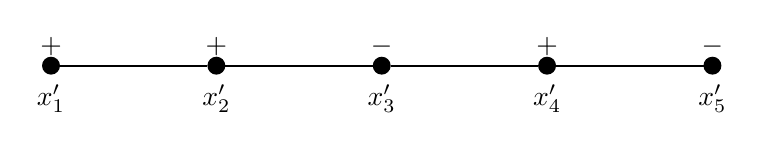
\begin{tikzpicture}[scale=1.4, thick]
        % Spine with sorted projections - simple black circles
        \node[draw, circle, fill=black, inner sep=2pt, label=below:$x'_1$] (X1) at (0,0) {};
        \node[draw, circle, fill=black, inner sep=2pt, label=below:$x'_2$] (X2) at (1.5,0) {};
        \node[draw, circle, fill=black, inner sep=2pt, label=below:$x'_3$] (X3) at (3,0) {};
        \node[draw, circle, fill=black, inner sep=2pt, label=below:$x'_4$] (X4) at (4.5,0) {};
        \node[draw, circle, fill=black, inner sep=2pt, label=below:$x'_5$] (X5) at (6,0) {};
        
        % Spine edges
        \draw (X1) -- (X2) -- (X3) -- (X4) -- (X5);
        
        % Highlight adjacent pairs
        \draw[thick] (X2) -- (X3);
        \draw[thick] (X4) -- (X5);
        
        % Class labels above nodes
        \node[above] at (X1) {$+$};
        \node[above] at (X2) {$+$};
        \node[above] at (X3) {$-$};
        \node[above] at (X4) {$+$};
        \node[above] at (X5) {$-$};
    \end{tikzpicture}
    \caption{Adjacency property: optimal support pairs are adjacent on spine.}
    \label{fig:adjacency}
\end{figure}

The adjacency property established in Theorem~\ref{thm:adjacency} is the cornerstone of our efficient algorithm. By restricting the search space to adjacent pairs on the spine, we reduce the problem from considering $O(n^2)$ potential support pairs to only $O(n)$ candidates. This dramatic reduction in complexity enables us to design practical algorithms with strong theoretical guarantees, as illustrated in \Cref{fig:adjacency}. % [LE: Added reference to adjacency figure]

\subsection{Algorithm and Complexity Analysis}
\label{subsec:algorithm}

In this section, we focus on the  design of an efficient algorithm for training SVM model on tree with $\lambda=1$.

% \subsubsection{Dynamic Programming for Objective Evaluation}

% To efficiently compute $f(u,v)$ for any pair $(u,v)$, we employ a dynamic programming approach using two depth-first search (DFS) passes along the branch $u \to v$:

% \begin{enumerate}
% \item \textbf{Size computation pass}: Root the tree $T$ at vertex $u$ and compute, for every node $a$, the subtree sizes:
% \begin{align}
% \mathrm{sz}_+(a) &= |\{z \in \text{subtree}(a) : y(z) = +1\}|, \\
% \mathrm{sz}_-(a) &= |\{z \in \text{subtree}(a) : y(z) = -1\}|.
% \end{align}

% \item \textbf{Distance accumulation pass}: Still with the tree rooted at $u$, accumulate the weighted distances:
% \begin{align}
% \mathrm{dist}_+(a) &= \sum_{\substack{z \in \text{subtree}(a)\\ y(z) = +1}} d(z,a), \\
% \mathrm{dist}_-(a) &= \sum_{\substack{z \in \text{subtree}(a)\\ y(z) = -1}} d(z,a).
% \end{align}

% These values are then combined along the unique path $u \to v$ to obtain $f_+(u,v)$. By symmetry, rooting the tree at $v$ yields $f_-(v,u)$.
% \end{enumerate}

% Since our augmented tree has a spine-and-spoke structure (essentially a path with leaves), all tree traversals can be performed in linear time.

\subsubsection{Algorithm and Complexity Analysis}


\begin{algorithm}[htbp]
\caption{SVM on Tree}
\label{alg:svm_tree}
\begin{algorithmic}[1]
\STATE \textbf{Input:} Labeled dataset $\{(x_i,y_i)\}_{i=1}^n \subset \mathbb{R}^d \times \{-1,+1\}$
\STATE \textbf{Output:} Optimal support pair $(s^*,p^*)$

\STATE Compute class means $\mu_-$, $\mu_+$ and spine direction $w$
\STATE Project all points: $x_i' = \mu_- + \langle x_i-\mu_-, w\rangle w$ for $i = 1,\ldots,n$
\STATE Sort projections $\{x_i'\}$ by coordinate $t_i = \langle x_i-\mu_-, w\rangle$
\STATE Construct augmented tree $T$ with spoke and spine edges (see Section~\ref{sec:tree-based-approximation}) % [LE: Added proper section reference]
\STATE Initialize $L_{\min} = \infty$ %, $(s^*,p^*) = \emptyset$
\STATE Compute $f(x'_i, x'_{i+1})$ for all $i=1,\ldots, n-1$ using preprocessing step in Section~\ref{sec:preprocessing} % [LE: Fixed ellipsis and added section reference]
\STATE Compute the total loss $L_1(x'_i, x'_{i+1}) = f(x'_i, x'_{i+1}) -d(x'_i, x'_{i+1})$ for all $i=1,\ldots, n-1$ % [LE: Fixed ellipsis]
\STATE Let $(s^*,p^*)=(x'_i, x'_{i+1})$ where $(x'_i, x'_{i+1})$ is  the pair with minimum total loss $L_1(x'_i, x'_{i+1})$ and $y_i\neq y_{i+1}$
% \FOR{$i=1,..., n-1$}
%     \STATE Let $(s,p) = (x'_i, x'_{i+1})$ with $y_i \neq y_{i+1}$
%     % \STATE Compute $f(s,p)$ using XXX and XXX
%     \STATE Calculate $L(s,p) = f(s,p) - d(s,p)$
%     \IF{$L(s,p) < L_{\min}$}
%         \STATE $L_{\min} = L(s,p)$
%         \STATE $(s^*,p^*) = (s,p)$
%     \ENDIF
% \ENDFOR

\STATE \textbf{return} $(s^*,p^*)$ % and perpendicular bisector of segment $s^*p^*$
\end{algorithmic}
\end{algorithm}


The computational complexity of our algorithm is analyzed as follows:

\begin{itemize}
\item \textbf{Projection step}: Computing projections for $n$ points in $\mathbb{R}^d$ requires $O(nd)$ operations.
\item \textbf{Sorting step}: Sorting $n$ projections by their coordinates takes $O(n \log n)$ time.
\item \textbf{Tree construction}: Building the augmented tree with $n$ spoke edges and $O(n)$ spine edges requires $O(n)$ time.
\item \textbf{Objective evaluation}: Each DFS traversal takes $O(n)$ time, and there are $O(n)$ adjacent pairs to evaluate due to Theorem~\ref{thm:adjacency}. % [LE: Replaced "step XXX" with specific description]
\end{itemize}

We finally obtain
\begin{theorem}[Complexity]
The overall time complexity of Algorithm~\ref{alg:svm_tree} is $O(nd + n \log n)$, or $O(n \log n)$ for fixed dimension $d$. \textcolor{blue}{[LE: Verified complexity claim]}
\end{theorem}

This represents a significant improvement over exhaustive search, which would require $O(n^2)$ pair evaluations (confirmed by adjacency property), each taking $O(n)$ time for objective computation. % [LE: Verified complexity claim]

% \subsubsection{Optimization Problem Statement}

% The core optimization problem solved by our algorithm is:

% \begin{problem}[SVM on Tree]
% Given the augmented tree $T$ and loss function $L(\cdot,\cdot)$, find:
% \[
% (s^*,p^*) = \arg\min_{(s,p): y(s) \neq y(p)} L(s,p) = \arg\min_{(s,p): y(s) \neq y(p)} [f(s,p) - d(s,p)].
% \]
% \end{problem}

% By Theorem~\ref{thm:adjacency}, this optimization reduces to considering only adjacent opposite-label projection pairs on the spine, dramatically reducing the search space from $O(n^2)$ to $O(n)$ candidates.
